\section{PCA}

Für die PCA berechnet man sich die Kovarianz-Matrix $C_X$ der Transponierten Datenmenge $X$. Aus $C_X$ berechnet man nun die Diagonal Matrix der Eigenwerte $EW$ und die Eigenvektoren $EV$.
Um die Projektion zu erhalten muss man die Spalte der Eigenvektoren, die Äquivalent zum Maximum der Eigenwert ist, transponieren und mit den Daten Multiplizieren.

\begin{figure}[h!]
  \begin{center}
    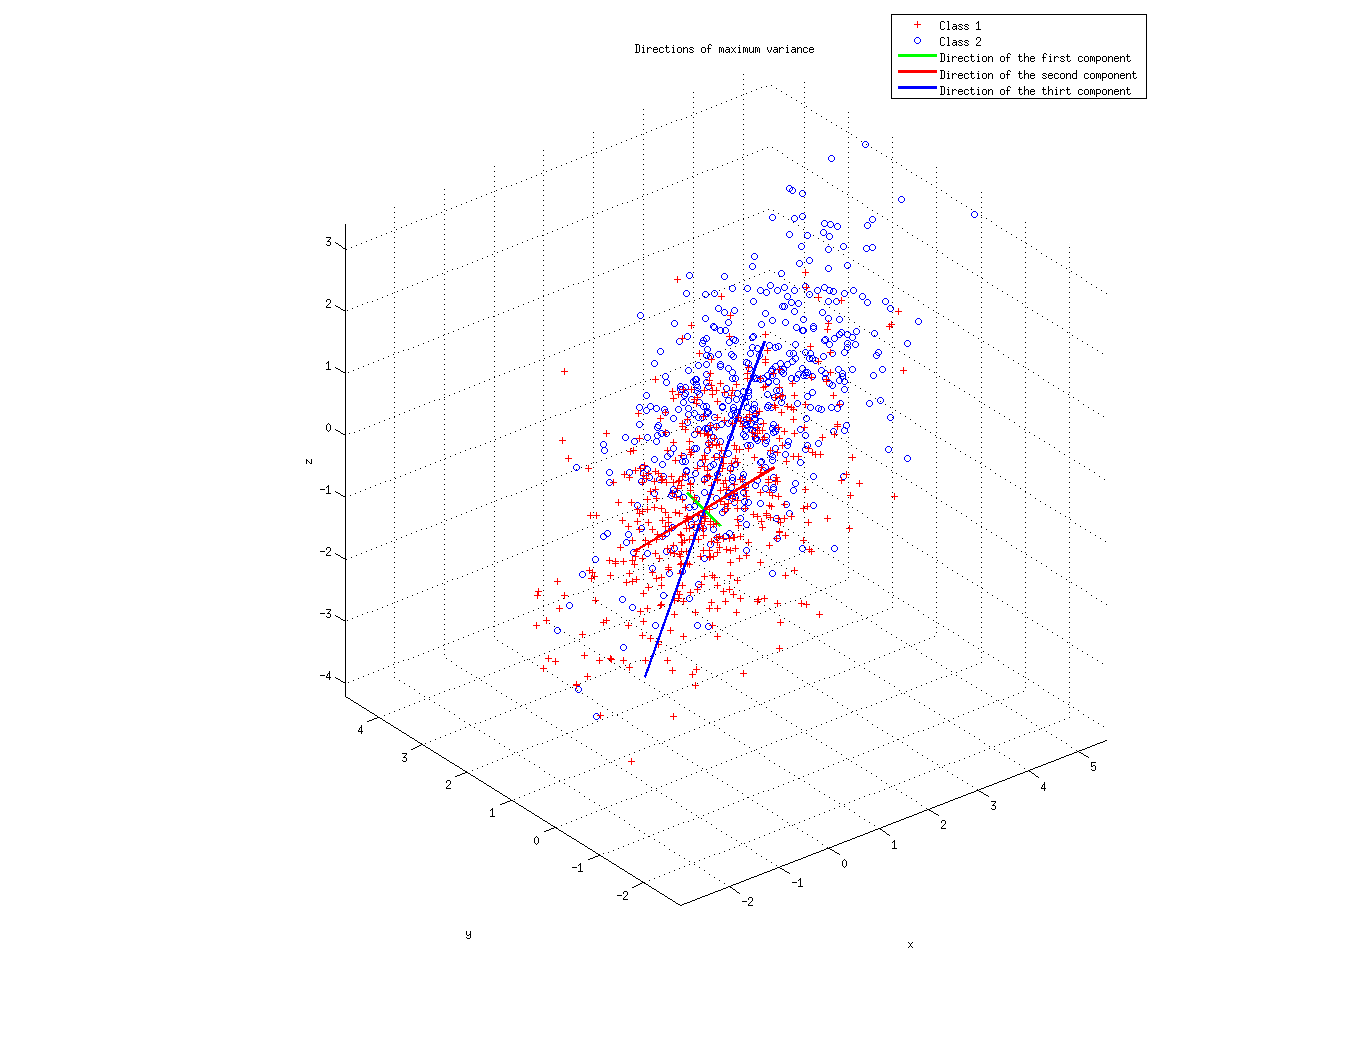
\includegraphics[width=1.0\textwidth]{./figures/4_Components}
    \caption{Die Richtungen der maximalen Varianz für die Daten, Richtungen mit den Eigenwerten Skaliert.}
    \label{fig:4_components}
  \end{center}
\end{figure}

\begin{figure}[h!]
  \begin{center}
    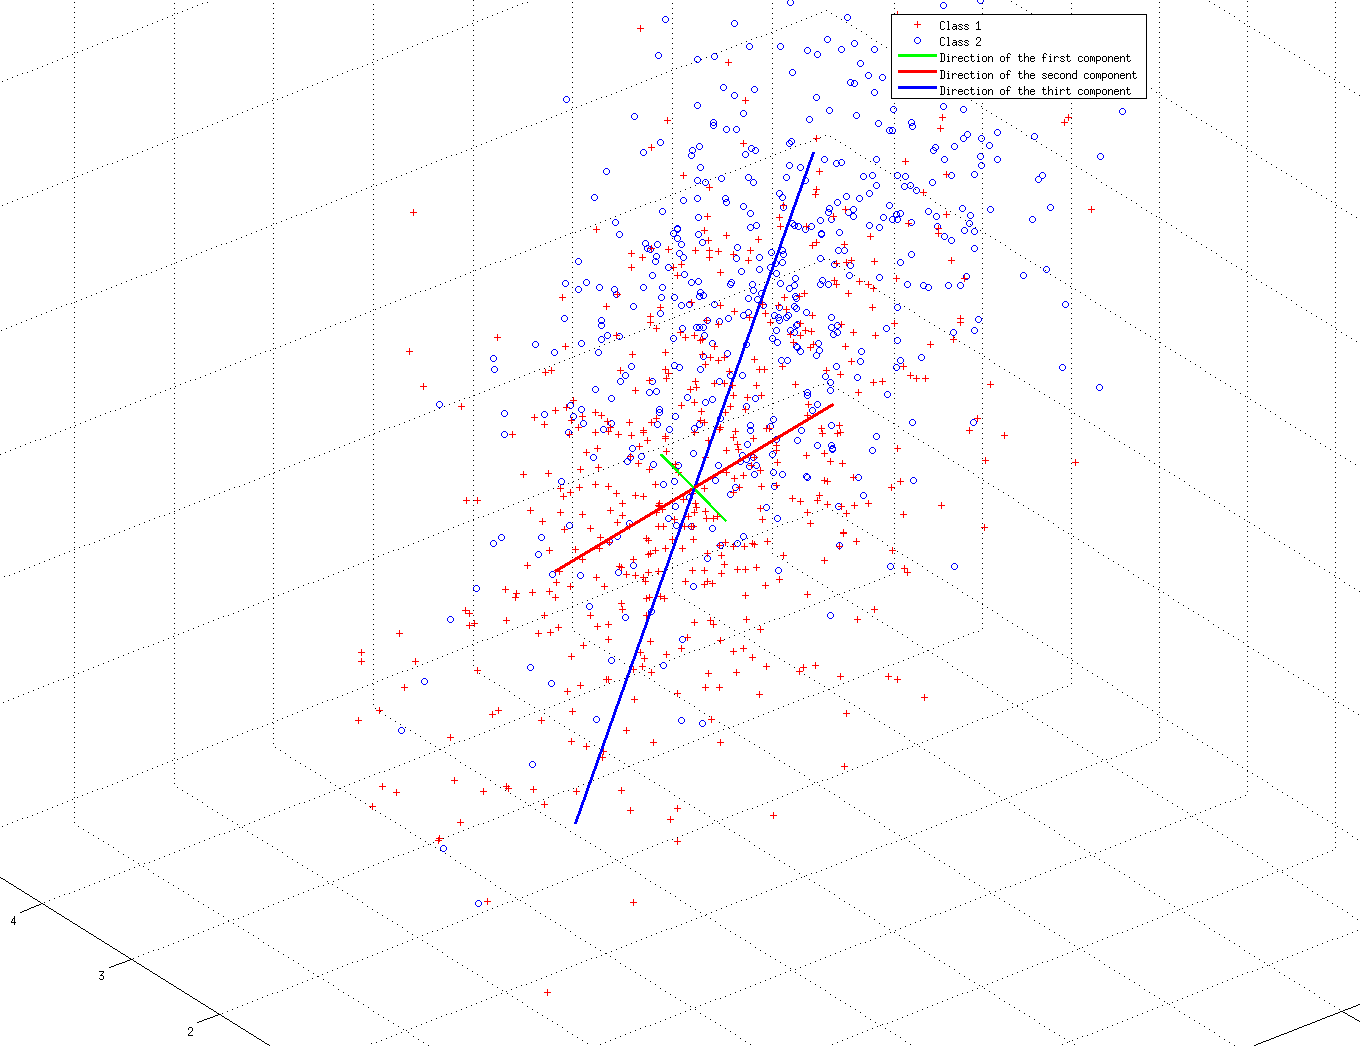
\includegraphics[width=1\textwidth]{./figures/4_Components_zoom}
    \caption{Die Richtungen der maximalen Varianz für die Daten, Richtungen mit den Eigenwerten Skaliert und vergrößert.}
    \label{fig:4_components_zoom}
  \end{center}
\end{figure}
Abbildung~\ref{fig:4_components} zeigt die Wolke aus den Punkten, wobei die Punkte der beiden Klassen getrennt dargestellt werden, und die zu den Daten gehörenden Hauptkomponenten.
Abbildung~\ref{fig:4_components_zoom} zeigt das selbe Bild nur etwas Vergrößert. Die Hauptrichtungen, wie man einigermaßen erkennen kann sind orthogonal zueinander.\newline
 
\begin{figure}[h!]
  \begin{center}
    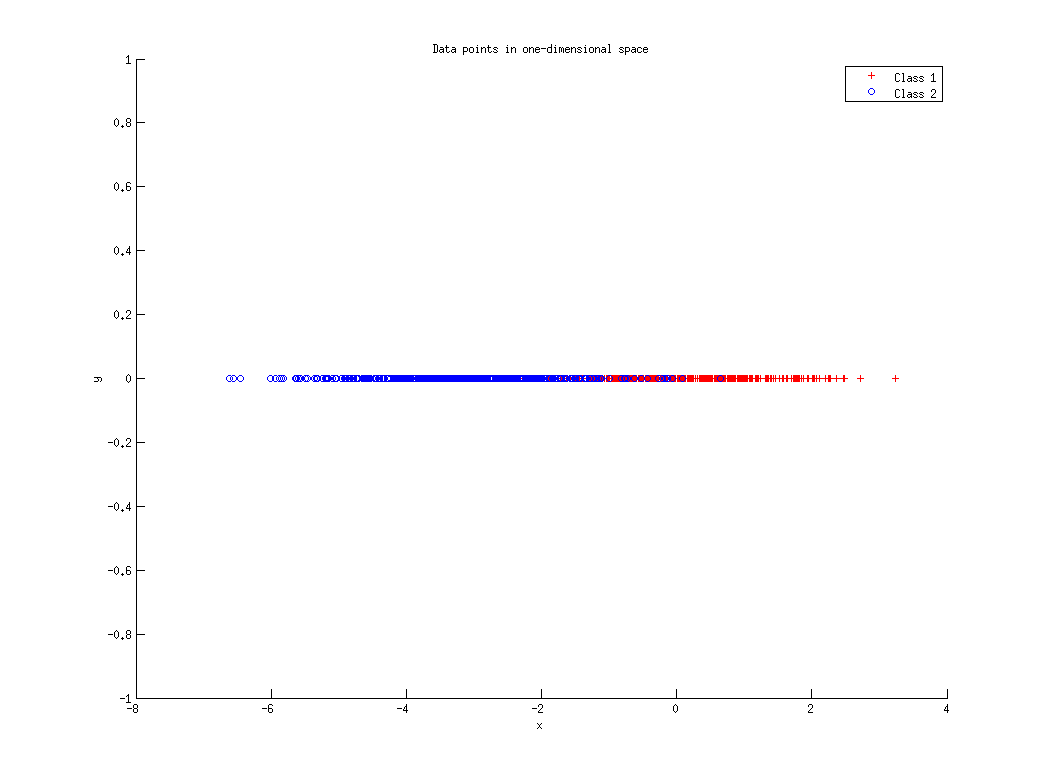
\includegraphics[width=0.75\textwidth]{./figures/4_one_dim}
    \caption{Projektion der Daten in eine einzige Dimension.}
    \label{fig:4_one_dim}
  \end{center}
\end{figure}

\begin{figure}[h!]
  \begin{center}
    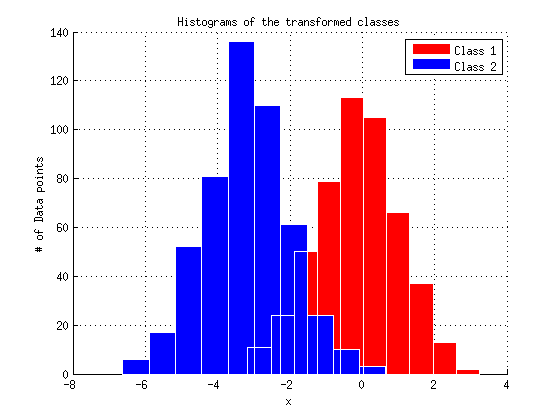
\includegraphics[width=0.75\textwidth]{./figures/4_Histogram}
    \caption{Histogram der Projezierten Daten.}
    \label{fig:4_Histogram}
  \end{center}
\end{figure}


Die Kovarianzmatrix ( $S_P = EV' * C_X * EV$ ) ist nach der PCA eine Diagonal-matrix. Die Werte sind nach der PCA dekorreliert aber nicht normalverteilt, da sie vor der Transformation auch nicht normalveteilt waren.\newline

Unser Threshold berechnet sich in unserem Beispiel zu -1.1983 die Performance liegt bei 88.5\% ( 81.6\% für die erste Klasse und 95.4\% für die Zweite Klasse).

